% !TEX TS-program = xelatex
% !TEX encoding = UTF-8 Unicode

% GSET Summer 2023 - Tennessee Technological University
% Tristan Hill - June 12, 2023
% Turtorial 6 - Conditionals

% matplotib and graphing 
% trigonometric functions
% logic and conditional statements 

\documentclass[12pt]{article}

% Custom Preamble
\usepackage{/mnt/c/Users/thill/Documents/courses/py_workshop/modules/py_tutorials}

% Title and Misc
\newcommand{\MNUM}{6} %Module Number
\newcommand{\MNAME}{Conditionals} %Module Name
\newcommand{\TNAME}{Triangles and Quadralaterals} %Tutorial Name
\pagestyle{myheadings}
\markright{{\large GSET - Introduction to Programming with Python}}

\begin{document}

    \thispagestyle{plain}

    \begin{center}
       {\bf \large GSET - Introduction to Programming with Python - Summer 2023} \vspace{5mm}\\
       {\bf \Large \MNAME \hspc -  Tutorial\hspc\MNUM\hspc - \TNAME}\vspace{3mm}\\      
    \end{center}

    %\Large
	\begin{description}[labelindent=1cm]

        \item [\textbf{\underline{Overview}}]\textbf{:} \\ 

        Scienctists and engineers benefit from the understanding of Trigonometry. In this exercise you are going to use the trigonometry tools available with NUMPY to solve a simple geometry problem and the graphing tools in MATPLOTLIB to display the results. You will also use conditional statements to determine the type of geometry of different examples.

        \item[\textbf{\underline{System Requirements:}}] \hfill \vspace{0mm}
        \begin{itemize}
            \item {\bf Computer}: A computer is required to complete this tutorial. Any OS should work.
            \item {\bf Python:} An online Python compiler that supports NumPY and MATPLOTLIB is required( \href{https://trinket.io/embed/python3/a5bd54189b}{Trinket Python3} ) or a Python system of your choice with NumPy and MATLPLOT installed.
        \end{itemize}

        \item [\textbf{\underline{Simple Geometry - Area of a Polygon}}]\textbf{:} \\

        You will be calculating the side length and area of a triangle and a quadrilateral (4 sided polygon). You have been given several formulas on the next page. \\

        \item [\textbf{\underline{Trigonometric Functions from NumPy}}]\textbf{:}\\\\ The trigonometric functions that you need are included in the \href{https://numpy.org/doc/stable/reference/routines.math.html}{NumPy Mathematics functions} list. To use NumPy, \lstinline{import numpy}.   

        \begin{itemize}             
            %\begin{multicols}{2}
            \item \lstinline{numpy.sin(x)} - sine of x
            \item \lstinline{numpy.cos(x)} - cosine of x
            \item \lstinline{numpy.tan(x)} - tangent of x

            \item \lstinline{numpy.asin()} - inverse aka arc-sine  
            \item \lstinline{numpy.acos()} - inverse aka arc-cosine
            \item \lstinline{nupy.atan()} - inverse aka arc-tangent
            %\end{multicols}
        \end{itemize}    

        \vspace{20mm}

        \newpage
        \item [\textbf{\underline{Equations}}]\textbf{:} \\
        \begin{itemize}             
            \item {\bf Distance Formula:} \scalebox{1}{$D_{ij}=\sqrt{(x_i-x_j)^2+(y_i-y_j)^2}$} \\

            \item {\bf Herons Formula(Area):} \scalebox{1}{$A=\sqrt{s(s-a)(s-b)(s-c)}$} \vspace{2mm}\\
            \item {\bf Perimeter Formula:} \scalebox{1}{$p = a+b+c$ and $s=p/2$} \vspace{2mm}\\
            \item {\bf Law of Cosines:} 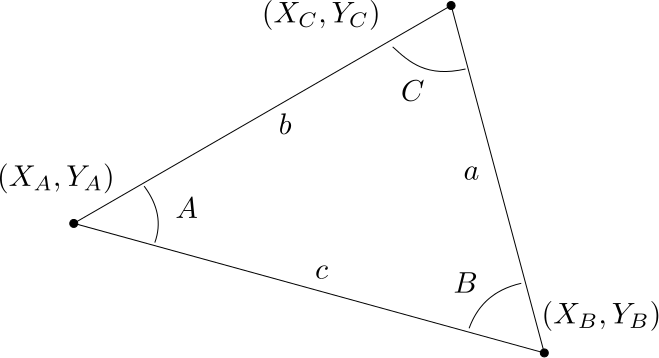
\includegraphics[scale=.5]{hw2_fig1.png} \\

            \scalebox{1}{$a^2 = b^2+c^2-2bc\times\cos(A)$} \vspace{2mm}\\
            \scalebox{1}{$b^2 = a^2+c^2-2ac\times\cos(B)$} \vspace{2mm}\\
            \scalebox{1}{$c^2 = a^2+b^2-2ab\times\cos(C)$} \vspace{2mm}\\   

            \item \textbf{Types of Triangles}
                \begin{itemize}
                \item Equilateral
                \item Right
                \item Isosceles
                \item Scalene
                \item Acute 
                \item Obtuse
                \end{itemize} 
        \end{itemize}
        
        \vspace{20mm}

        \newpage
        \item [\textbf{\underline{Program Minimum Requirements:}}] The program should accomplish the following tasks.
        %\begin{description}
        \begin{enumerate}
        \item Ask the user to enter the 3 vertices of a triangle using the {\it input()} function. The data should be stored using lists. Give the user instructions for correctly entering the data. \\
        \item Show the vertices as points and the legs of the triangle as lines using MATPLOTLIB. Choose your own markers and linetypes.  \\
        \item Calculate the length of each side of the triangle. Show these results in the command window with {\it print()}. \\
        \item Calculate each of the internal angles of the triangle. Show these results in the command window  with {\it print()}. \\  
        \item Calculate the area of the triangle. Show this result in the command window  with {\it print()}. \\  
        \item Use one or more conditional statements to determine what type of triangle is formed by the three points. There are six categories shown with the equations. Your program should print the category to the command window. \\
        
        \end{enumerate}

        \item [\textbf{\underline{Optional Advanced Features:}}] Add the following optional features if you have time. 
        \begin{enumerate}
            \item Check the input string for the correct number of values and format as requested by input() prompt. If there is a problem with the input, print an error message. Skip the calculations and end the program.
            \item Check the input string for the correct number of values and format as requested by input() prompt. If there is a problem with the input, print an error message. Skip the calculations and repeat the process allowing the user to input a new string. The program should not end until the correct input has been recieved and the calculations have been completed. 
        \end{enumerate} 
       



        %			\item[Part 2]\textbf{: Quadrilateral}
        %			\begin{enumerate}
        %				\item Ask the user to enter the 4 vertices of a quadrilateral using the {\it input()} function. The data should be stored into 2 separate arrays, 1 array for x data and 1 array for y data.  \\
        %\item Show the quadrilateral using the plot function. \\
        %                \item Calculate the length of each side of the shape. Also, calculate the length of 1 or both of the {\it diagonals}. Show these results in the command window with {\it fprintf()}. \\
        %		\item Calculate each of the internal angles of the quadrilateral. Show these results in the command window  with {\it fprintf()}.  \\
        %			\item Calculate the area of the quadrilateral. Show this result in the command window  with {\it fprintf()}. \\  
        %	
        %			\end{enumerate}

        \item[\textbf{\underline{Example Code:}}] \hfill \vspace{0mm}

        %\begin{minted}{cpp}
        \begin{lstlisting}
# Condtionals - GSET - Summer 2023 

# prompt the user for input
data=input('''Type the values for the vertices of a triangle
The following format is required. x1, y1, x2, y2, x3, y3:''')

# get values from user input, store as separate lists 
xvals=[float(data.split(',')[0]), float(data.split(',')[2]), float(data.split(',')[4])]
yvals=[float(data.split(',')[1]), float(data.split(',')[3]), float(data.split(',')[5])]
print('xvalues:',xvals)
print('yvalues:',yvals)

        \end{lstlisting}
        %\end{minted}

\newpage
        \item[\textbf{\underline{Testing:}}] \hfill \vspace{0mm}
        \begin{enumerate}

        \item Complete the Python code to the solve the problem described. \\\\

        \item Test your code with different inputs. Is the answer correct? How do you know? Are there certain inputs that do not work? \\\\

        \item Save your code with the download button or use copy and paste. You can view and edit the code in any text editor. Also, save a copy of the program output for your tutorial summary. \\\\

        \end{enumerate}

        \item[\textbf{\underline{Solution Code:}}] \hfill \vspace{0mm}

        \begin{lstlisting}

        COMING SOON

        \end{lstlisting}

        \item[\textbf{\underline{Tutorial Summary:}}] \hfill \vspace{3mm}\\ 
        Write a brief summary of what you accomplished and what you struggled with the most. 

        Include the following items in the summary:
        \begin{itemize}

        \item a copy of the output of your program
        \item a description of what the program does and how to use it

        \end{itemize}


        \item[\textbf{\underline{Submission:}}] \hfill \vspace{3mm}\\ 
        Use the appropriate assignment folder on ilearn to submit your program and summary. Submit the following items with your TNTech username in the filenames as shown below. \vspace{0mm}\\

        \underline{Files for Tutorial \MNUM\ (TNTech Username : twhill21)}

        \begin{itemize}

        \item Tutorial Summary: \textbf{ twhill21\_summary\MNUM .txt}

        \item Python Source Code: \textbf{ twhill21\_tutorial\MNUM .py}

        \end{itemize}

        \item[\textbf{\underline{Tutorial Complete:}}] \hfill \vspace{3mm}\\ 
        Congratulations, after completing {\it Tutorial\_\MNUM\_\TNAME}, you have learned to use conditional statements in Python! You are now ready to start learning about iterative program flow. \\

    \end{description}
 
\end{document}



